\documentclass[12pt,twoside]{article}
\usepackage[utf8]{inputenc}
\usepackage[english,russian]{babel}
\usepackage{abstract}
\usepackage{amsmath,amssymb,mathrsfs,mathtext,amsthm}
\usepackage{a4wide}
\usepackage[T2A]{fontenc}
\usepackage{subfig}
\usepackage{url}
\usepackage[usenames]{color}
\usepackage{colortbl}

\newcommand{\hdir}{.}
\usepackage{hyperref}       % clickable links
\usepackage{lineno}
\usepackage{graphicx,multicol}
\usepackage{epstopdf}
\usepackage{cite}
\usepackage{amsmath,amssymb,mathrsfs,mathtext}
\usepackage{tikz}
\usetikzlibrary{shapes,arrows,shadows}
\newtheorem{theorem}{Теорема}
\newtheorem{statement}{Утверждение}
\usepackage{algorithm}
\usepackage[noend]{algcompatible}

%\renewcommand{\baselinestretch}{1.4}


\newcommand{\bx}{\mathbf{x}}
\newcommand{\by}{\mathbf{y}}
\newcommand{\bw}{\mathbf{w}}
\newcommand{\bY}{\mathbf{Y}}
\newcommand{\bX}{\mathbf{X}}
\newcommand{\bu}{\mathbf{u}}
\newcommand{\bt}{\mathbf{t}}
\newcommand{\bp}{\mathbf{p}}
\newcommand{\bq}{\mathbf{q}}
\newcommand{\bc}{\mathbf{c}}
\newcommand{\bP}{\mathbf{P}}
\newcommand{\bT}{\mathbf{T}}
\newcommand{\bQ}{\mathbf{Q}}
\newcommand{\bC}{\mathbf{C}}
\newcommand{\bE}{\mathbf{E}}
\newcommand{\bF}{\mathbf{F}}
\newcommand{\bU}{\mathbf{U}}
\newcommand{\bW}{\mathbf{W}}
\newcommand{\btheta}{\boldsymbol{\theta}}
\newcommand{\bTheta}{\boldsymbol{\Theta}}
\newcommand{\T}{^{\text{\tiny\sffamily\upshape\mdseries T}}}

\begin{document}
	\title
	{Снижение размерности в задачах декодирования временных рядов и прогнозирования\thanks{Работа выполнена при финансовой поддержке РФФИ (проект 16-07-01155).}}
	\date{}
	\maketitle
	\begin{center}
		Р.\,В.~Исаченко\footnote{Московский физико-технический институт, isa-ro@yandex.ru},
		М.\,Р.~Владимирова\footnote{Московский физико-технический институт, vladimirova.maria@phystech.edu},
		В.\,В.~Стрижов\footnote{Вычислительный центр им. А. А. Дородницына ФИЦ ИУ РАН, strijov@ccas.ru}
	\end{center}
	\textbf{Аннотация:} Решается задача обнаружения зависимостей в прогнозируемой переменной. 
	Вместо построения прогноза одного момента времени предлагается прогнозировать многомерный вектор прогноза.
	Рассматривается линейная модель метода частных наименьших квадратов. 
	Описан метод нахождения матрицы совместного описания для исходных матриц объектов и ответов. 
	Найденное описание является низкоразмерным, что позволяет построить устойчивую, простую модель.
	Проводится вычислительный эксперимент на реальных данных объемов потребления электроэнергии и данных сигналов кортикограмм.
	
	\bigskip
	\textbf{Ключевые слова}: декодирование временных рядов; метод частных наименьших квадратов; PLS; снижение размерности

\linenumbers
%%%%%%%%%%%%%%%%%%%%%%%%%%%%%%%%%%%%%%%%%%%%%%%%%%%%%%%%%%%%%%%%%%%%%%%%%%%%%%
\section{Введение}
%%%%%%%%%%%%%%%%%%%%%%%%%%%%%%%%%%%%%%%%%%%%%%%%%%%%%%%%%%%%%%%%%%%%%%%%%%%%%%

В работе рассматривается задача восстановления зависимости между независимой и прогнозируемой переменными.
Предлагаемая модель позволяет восстанавливать зависимость в случае многомерной прогнозируемой переменной. 
В случае задачи прогнозирования пространства объектов и ответов имеют одну и ту же природу.
Для построения модели по исходному временному ряду строятся авторегрессионные матрицы объектов и ответов. 
Объектом является локальная история сигнала, ответом~--- значение сигнала в следующие моменты времени.
Авторегрессионная модель предполагает, что значение сигнала в данный момент времени линейно зависит от предыдущих значений этого же сигнала.   

В задаче декодирования временных рядов пространство объектов имеет значимо большую размерность. В этом случае пространства объектов и ответом имеют разную природу, ответом является отклик системы на входной сигнал. Авторегрессионная матрица объектов содержит локальную историю входного сигнала, а авторегрессионная матрица ответов содержит локальную историю отклика.

Исходное признаковое пространство является многомерным. Избыточная размерность признакового пространства приводит к неустойчивости модели.
Для решения этой проблемы используются методы отбора признаков~\cite{katrutsa2015qpfs,li2016feature}.

В работе исследуется метод частных наименьших квадратов (PLS) \cite{wegelin2000survey,abdi2003pls,geladi1986partial}.
Метод частных наименьших квадратов снижает размерности матрицы признаков и выделяет линейные комбинации признаков, которые оказывают наибольшее влияние на вектор ответов. 
Выделение признаков происходит итеративно, в порядке уменьшения их влияния на вектор ответов. Рассматриваются только значимые комбинации признаков, незначительно потеряв в точности прогноза. 
Методы PLS регрессии подробно описаны в работах~\cite{geladi1988pls, hoskuldsson1988plsr,de1993simpls}. 
Разницу между методом PLS и связанными с ним подходами, различные разновидности регрессии PLS можно найти в~\cite{rosipal2006overview}.

Современное состояние области и обзор нелинейных модификаций метода PLS описаны~\cite{rosipal2011npls}.
Нелинейное расширение метода PLS регрессии впервые введено в~\cite{wold1989nonlinear}. 
В литературе были разработаны различные модификации PLS. 
Предложены нелинейные методы PLS, основанные на различных моделях: 
сглаживающих сплайнах~\cite{frank1990npls} нейронных сетях~\cite{qin1992npls}, базисных радиальных функциях~\cite{yan2003geneticpls}, генетическом алгоритме~\cite{hiden1998geneticpls}. 

Результатом отбора признаков является снижение размерности задачи и повышение устойчивости моделей без существенной потери точности прогноза.
Методы решения задачи сравниваются на двух наборах данных, имеющих избыточную информацию. 
Первый набор данных~--- почасовые временные ряды объёмов потребления электроэнергии. Временные ряды соответствуют периоду 1999-2004 годов. 

Второй набор данных взят из проекта NeuroTycho~\cite{neurotycho}, в котором проектируется нейрокомпьютерный интерфейс (BCI)~\cite{millan2010combining,mason2007comprehensive} для обмена информацией между мозгом и электронным устройством. 
Система BCI повышает умственные и физические способности пользователя, обеспечивая прямую связь между мозгом и компьютером~\cite{millan2004brain}. 
BCI восстановливает поврежденную функциональность пациентов с нарушениями двигательного или когнитивного развития. 
Цель анализа моторных изображений заключается в распознавании предполагаемых движений по записанной активности мозга. 
Существуют различные методы измерения кортикальных данных для BCI описанные в~\cite{nicolas2012brain,amiri2013review}. 
В работе рассматриваются сигналы электрокортикографии (ECoG)~\cite{eliseyev2016penalized}. ECoG, как и другие инвазивные методы, обеспечивает более стабильную запись и лучшее разрешение в временных и пространственных областях, чем ее неинвазивные аналоги.
Данные ECoG являются многомерными и измерения коррелируют как во временной, так и в пространственной областях.
Задача состоит в предсказании траектории движения руки по временным рядам напряжения кортикальной активности. 
Сигналы ECoG измеряются через 32 канала, в то время как субъект перемещает руку. 

В работах по прогнозированию сложных пространственных временных рядов прогноз выполняется поточечно.
При необходимости прогнозировать несколько точек одновременно задачу предлагается решать последовательно вычисляя прогноз по точкам. При этом используются предыдущие спрогнозированные значения для получения последующих.
Предлагаемый метод позволяет получать временной ряд прогнозируемых значений одновременно с учётом скрытых зависимостей не только в пространстве объектов, но и в пространстве ответов с согласованием этих двух зависимостей.
Предлагаемый метод позволил существенно снизить размерность признакового пространства. 
 
%%%%%%%%%%%%%%%%%%%%%%%%%%%%%%%%%%%%%%%%%%%%%%%%%%%%%%%%%%%%%%%%%%%%%%%%%%%%%%

\section{Постановка задачи}
%%%%%%%%%%%%%%%%%%%%%%%%%%%%%%%%%%%%%%%%%%%%%%%%%%%%%%%%%%%%%%%%%%%%%%%%%%%%%%
Задана выборка $\mathfrak{D}= \left( \bX, \bY \right)$, где $\mathbf{X} \in \mathbb{R}^{m \times n}$~--- матрица объектов, $\mathbf{Y} \in \mathbb{R}^{m \times r}$~--- матрица ответов. 
Способ построения выборки под определенную прикладную задачу описан в разделе \textit{Вычислительный эксперимент}.

Предполагается, что между объектами $\bx \in \mathbb{R}^n$ и ответами $\by \in \mathbb{R}^r$ существует линейная зависимость 
\begin{equation}
 \underset{1 \times r}{\by} = \underset{1 \times n}{\vphantom{\by}\bx} \cdot \underset{n \times r}{\vphantom{\by}\bTheta} + \underset{1 \times r}{\vphantom{\by}\boldsymbol{\varepsilon}}, 
\label{eq::model}
\end{equation}
где $\bTheta$~---~матрица параметров модели, а~$\boldsymbol{\varepsilon}$~---~вектор регрессионных остатков.

Необходимо по известной выборке $\mathfrak{D}$ восстановить матрицу параметров модели~\eqref{eq::model}.
Оптимальные параметры находятся минимизацией функции ошибки.
Введем квадратичную функцию ошибки $S$ на выборке $\mathfrak{D}$:
\begin{equation}
	S(\bTheta | \mathfrak{D}) = {\bigl\| \underset{m \times n}{\vphantom{\by}\mathbf{X}} \cdot \underset{n \times r}{\vphantom{\by}\bTheta} - \underset{m \times r}{\vphantom{\by}\mathbf{Y}} \bigr\| }_2^2 = \sum_{i=1}^m \| \underset{1 \times n}{\vphantom{\by}\bx_i} \cdot \underset{n \times r}{\vphantom{\by}\bTheta} - \underset{1 \times r}{\vphantom{\by}\by_i} \|_2^2 \rightarrow\min_{\bTheta}.
\label{eq::error_function}
\end{equation}
 
Линейная зависимость столбцов матрицы $\bX$ приводит к неустойчивому решению задачи оптимизации~\eqref{eq::error_function}. Для устранения линейной зависимости применяются методы отбора признаков.

\section{Метод частных наименьших квадратов}

Для устранения линейной зависимости и снижения размерности пространства применяется метод главных компонент PCA. 
Основным недостатком данного метода является то, что он не учитывает взаимосвязь между объектами и ответами.
Метод частных наименьших квадратов PLS проецирует матрицу объектов $\bX$ и матрицу ответов $\bY$ в латентное пространство $\mathbb{R}^l$ меньшей размерности ($l < r < n$).
Алгоритм PLS находит в латентном пространстве матрицу $\bT \in \mathbb{R}^{m \times l}$, наилучшим образом описывающую исходные матрицы $\bX$ и $\bY$.

Матрица объектов $\bX$ и матрица ответов $\bY$ проецируются в латентное пространство следующим образом: 
\begin{align}
\label{eq::PLS_X}
 \underset{m \times n}{\vphantom{\bQ}\bX} 
 &= \underset{m \times l}{\vphantom{\bQ}\bT} \cdot \underset{l \times n}{\vphantom{\bQ}\bP^{\T}} + \underset{m \times n}{\vphantom{\bQ}\bF} 
 = \sum_{k=1}^l \underset{m \times 1}{\vphantom{\bp_k^{\T}}\bt_k} \cdot \underset{1 \times n}{\bp_k^{\T}} + \underset{m \times n}{\vphantom{\bp_k^{\T}}\bF},\\
 \label{eq::PLS_Y}
 \underset{m \times r}{\vphantom{\bQ}\bY} 
 &= \underset{m \times l}{\vphantom{\bQ}\bT} \cdot \underset{l \times r}{\bQ^{\T}} + \underset{m \times r}{\vphantom{\bQ}\bE}
 =  \sum_{k=1}^l  \underset{m \times 1}{\vphantom{\bq_k^{\T}}\bt_k} \cdot \underset{1 \times r}{\bq_k^{\T}} +  \underset{m \times r}{\vphantom{\bq_k^{\T}}\bE},
\end{align}
где $\bT$~--- матрица совместного описания объектов и ответов в латентном пространстве, причём столбцы матрицы $\bT$ ортогональны; $\bP,\ \bQ$~--- матрицы перехода из латентного пространства в  исходные пространства; $\bE,\ \bF$~--- матрицы невязок. 

Псевдокод метода регрессии PLS приведен в алгоритме~\ref{PLSR_code}.
Алгоритм итеративно на каждом из $l$ шагов вычисляет по одному столбцу $\bt_k$, $\bp_k$, $\bq_k$ матриц $\bT$, $\bP$, $\bQ$ соответственно. После вычисления следующего набора векторов из матриц $\bX$, $\bY$ вычитаются очередные одноранговые аппроксимации. 
Первым шагом необходимо произвести нормировку столбцов исходных матриц (вычесть среднее и разделить на стандартное отклонение).
На этапе тестирования необходимо провести нормировку тестовых данных, вычислить предсказание модели~\ref{eq::model}, а затем провести обратную нормировку.

\begin{algorithm}[h]
\caption{Алгоритм PLSR}
\label{PLSR_code}
\begin{algorithmic}[1]
	\REQUIRE $\bX, \bY, l$;
	\ENSURE $\bT, \bP, \bQ$;
	\STATE нормировать матрицы $\bX$ и $\bY$ по столбцам
	\STATE инициализировать $\bu_0$ (первый столбец матрицы $\bY$)
	\STATE $\bX_1 = \bX; \bY_1 = \bY$
	\FOR{$k=1,\dots, l$}
	\REPEAT
	\vspace{0.1cm}
	\STATE $\bw_k := \bX_k^{\T} \bu_{k-1} / (\bu_{k-1}^{\T} \bu_{k-1}); \quad \bw_k: = \frac{\bw_k}{\| \bw_k \|}$
	\vspace{0.1cm}
	\STATE $\bt_k := \bX_k \bw_k$
	\vspace{0.1cm}
	\STATE $\bc_k := \bY_k^{\T} \bt_k / (\bt_k^{\T} \bt_k); \quad \bc_k: = \frac{\bc_k}{\| \bc_k \|}$
	\vspace{0.1cm}
	\STATE $\bu_k := \bY_k \bc_k$
	\UNTIL{$\bt_k$ не стабилизируется}
	\vspace{0.1cm}
	\STATE $\bp_k:= \bX_k^{\T}\bt_k/(\bt_k^{\T}\bt_k),\ 
	\bq_k := \bY_k^{\T}\bt_k/(\bt_k^{\T}\bt_k)$
	\vspace{0.2cm}
	\STATE $\bX_{k+1} :=  \bX_k - \bt_k \bp_k^{\T}$
	\vspace{0.2cm}
	\STATE $\bY_{k + 1} :=  \bY_k - \bt_k \bq_k^{\T}$ 
	\ENDFOR
\end{algorithmic}
\end{algorithm}
Вектора $\bt_k$ и $\bu_k$ из внутреннего цикла алгоритма~\ref{PLSR_code}
содержат информацию о матрице объектов $\bX$ и матрице ответов $\bY$ соответственно. 
Блоки из шагов (6)-(7) и шагов (8)-(9)~--- аналоги алгоритма PCA для матриц $\bX$ и $\bY$~\cite{geladi1986partial}. 
Последовательное выполнение блоков позволяет учесть взаимную связь между матрицами $\bX$ и $\bY$.

Теоретическое обоснование алгоритма PLS следует из следующих утверждений.
\begin{statement}
Наилучшее описание матриц $\bX$ и $\bY$ с учётом их взаимосвязи достигается при максимизации ковариации между векторами $\bt_k$ и $\bu_k$. 
\end{statement}
Утверждение следует из равенства
\[
\text{cov} (\bt_k, \bu_k) = \text{corr} (\bt_k, \bu_k) \cdot \sqrt{\text{var}(\bt_k)} \cdot \sqrt{\text{var}(\bu_k)}.
\]
Максимизация дисперсий векторов $\bt_k$ и $\bu_k$ отвечает за сохранение информации об исходных матрицах, 
корреляция между векторами отвечает взаимосвязи между $\bX$ и~$\bY$. $\blacksquare$

Во внутреннем цикле алгоритма вычисляются нормированные вектора весов $\bw_k$ и $\bc_k$. Из данных векторов строятся матрицы весов $\bW$ и $\bC$ соответственно.

\begin{statement}
	В результате выполнения внутреннего цикла вектора $\bw_k$ и $\bc_k$ будут собственными векторами матриц $\bX_k^{\T} \bY_k \bY_k^{\T} \bX_k$ и $\bY_k^{\T} \bX_k \bX_k^{\T} \bY_k$, соответствующими максимальным собственным значениям.
	
	\begin{equation*}
	\bw_k \varpropto \bX_k^{\T} \bu_{k-1} \varpropto \bX_k^{\T} \bY_k \bc_{k-1} \varpropto \bX_k^{\T} \bY_k \bY_k^{\T} \bt_{k-1} \varpropto \bX_k^{\T} \bY_k \bY_k^{\T} \bX_k \bw_{k-1},
	\end{equation*}
	\begin{equation*}
	\bc_k \varpropto \bY_k^{\T} \bt_k \varpropto \bY_k^{\T} \bX_k \bw_k \varpropto \bY_k^{\T} \bX_k \bX_k^{\T} \bu_{k-1} \varpropto \bY_k^{\T} \bX_k \bX_k^{\T} \bY_k \bc_{k-1},
	\end{equation*}
	где символ $\varpropto$ означает равенство с точностью до мультипликативной константы. 
	\label{st::eig}
\end{statement}

Утверждение следует из того факта, что правила обновления векторов $\bw_k$, $\bc_k$ совпадают с итерацией алгоритма поиска максимального собственного значения. Данный алгоритм основан на следующем факте.

Если матрица $\mathbf{A}$ диагонализуема, $\bx$~--- некоторый вектор, то

\[
	\lim_{k \rightarrow \infty} \mathbf{A}^k \bx = \lambda_{\max}(\mathbf{A}) \cdot \mathbf{v}_{\max},
\]
где $ \lambda_{\max} (\mathbf{A})$~--- максимальное собственное значение матрицы $\mathbf{A}$, $\mathbf{v}_{\max}$~---собственный вектор матрицы $\mathbf{A}$, соответствующий $ \lambda_{\max} (\mathbf{A})$.
$\blacksquare$

\begin{statement}
Обновление векторов по шагам (6)--(9) алгоритма~\ref{PLSR_code} соответствует максимизации ковариации между векторами $\bt_k$ и $\bu_k$.
\end{statement}
Максимальная ковариация между векторами $\bt_k$ и $\bu_k$ равна максимальному собственному значению матрицы $\bX_k^{\T} \bY_k \bY_k^{\T} \bX_k$:
\begin{align*}
\max_{\bt_k, \bu_k}  \text{cov} (\bt_k, \bu_k)^2 &= \max_{\substack{\|\bw_k\|=1 \\ \|\bc_k\| = 1}} \text{cov} \left( \bX_k \bw_k, \bY_k \bc_k \right)^2 = \max_{\substack{\|\bw_k\|=1 \\ \|\bc_k\| = 1}} \text{cov} \left(\bc_k^{\T}  \bY_k^{\T} \bX_k \bw_k \right)^2 = \\
&= \max_{\|\bw_k\| = 1} \text{cov} \left\|\bY_k^{\T} \bX_k \bw_k \right\|^2 = \max_{\|\bw_k\| = 1} \bw_k^{\T} \bX_k^{\T} \bY_k \bY_k^{\T} \bX_k \bw_k = \\
& = \lambda_{\max} \left( \bX_k^{\T} \bY_k \bY_k^{\T} \bX_k \right),
\end{align*}
где $ \lambda_{\max} (\mathbf{A})$~--- максимальное собственное значение матрицы $\mathbf{A}$.
Применяя утверждение~\ref{st::eig}, получаем требуемое.
$\blacksquare$

После завершения внутреннего цикла на шаге (11) вычисляются вектора $\bp_k$, $\bq_k$ проецированием столбцов матриц $\bX_k$ и $\bY_k$ на вектор $\bt_k$. Для перехода на следующий шаг необходимо вычесть из матриц $\bX_k$ и $\bY_k$ одноранговые аппроксимации $\bt_k \bp_k^{\T}$ и $\bt_k \bq_k^{\T}$
\begin{equation*}
    \bX_{k + 1} = \bX_{k} - \bt_k \bp_k^{\T} = \bX - \sum_k \bt_k \bp_k^{\T},
\end{equation*}
\begin{equation*}
    \bY_{k + 1} = \bY_{k} - \bt_k \bq_k^{\T} = \bY - \sum_k \bt_k \bq_k^{\T}.
\end{equation*}
Тогда каждый следующий вектор $\bt_k$ оказывается ортогонален всем векторам $\bt_i$, $i=1, \dots, k$.

На Рис.~\ref{fig::PLSFigure} продемонстрирован результат работы алгоритма PLS для случая, когда размерности пространств объектов, ответов и латентного пространства равны 2 ($n = r = l = 2$).
Синими и зелёными точками изображены строки матриц $\bX$ и $\bY$. 
Точки были сгенерированы из нормального распределения с нулевым матожиданием. 
Красным контуром показаны линии уровня матриц ковариаций распределений. 
Черным изображены единичные окружности. 
Красные стрелки соответствуют главным компонентам. 
Черные стрелки соответствуют векторам матриц $\bW$ и $\bC$ алгоритма PLS. 
Вектора $\bt_k$ и $\bu_k$ равны проекциям матриц $\bX_k$ и $\bY_k$ на вектора $\bw_k$ и $\bc_k$ соответственно и изображены черными плюсами. 
Учёт взаимной связи между матрицами $\bX$ и $\bY$ отклоняет вектора $\bw_k$ и $\bc_k$ от направления главных компонент. 
Вектора $\bw_k$ отклоняются незначительно. 
На первой итерации $\bc_1$ близок к $\textit{pc}_1$, но вектора $\bc_k$, найденные на следующих итерациях могут оказаться сильно коррелированными. Это происходит в следствие того, что из матрицы $\bY$ на каждом шаге вычитается одноранговая аппроксимация, найденная в пространстве матрицы $\bX_k$.
\begin{figure}[h]
	\centering
	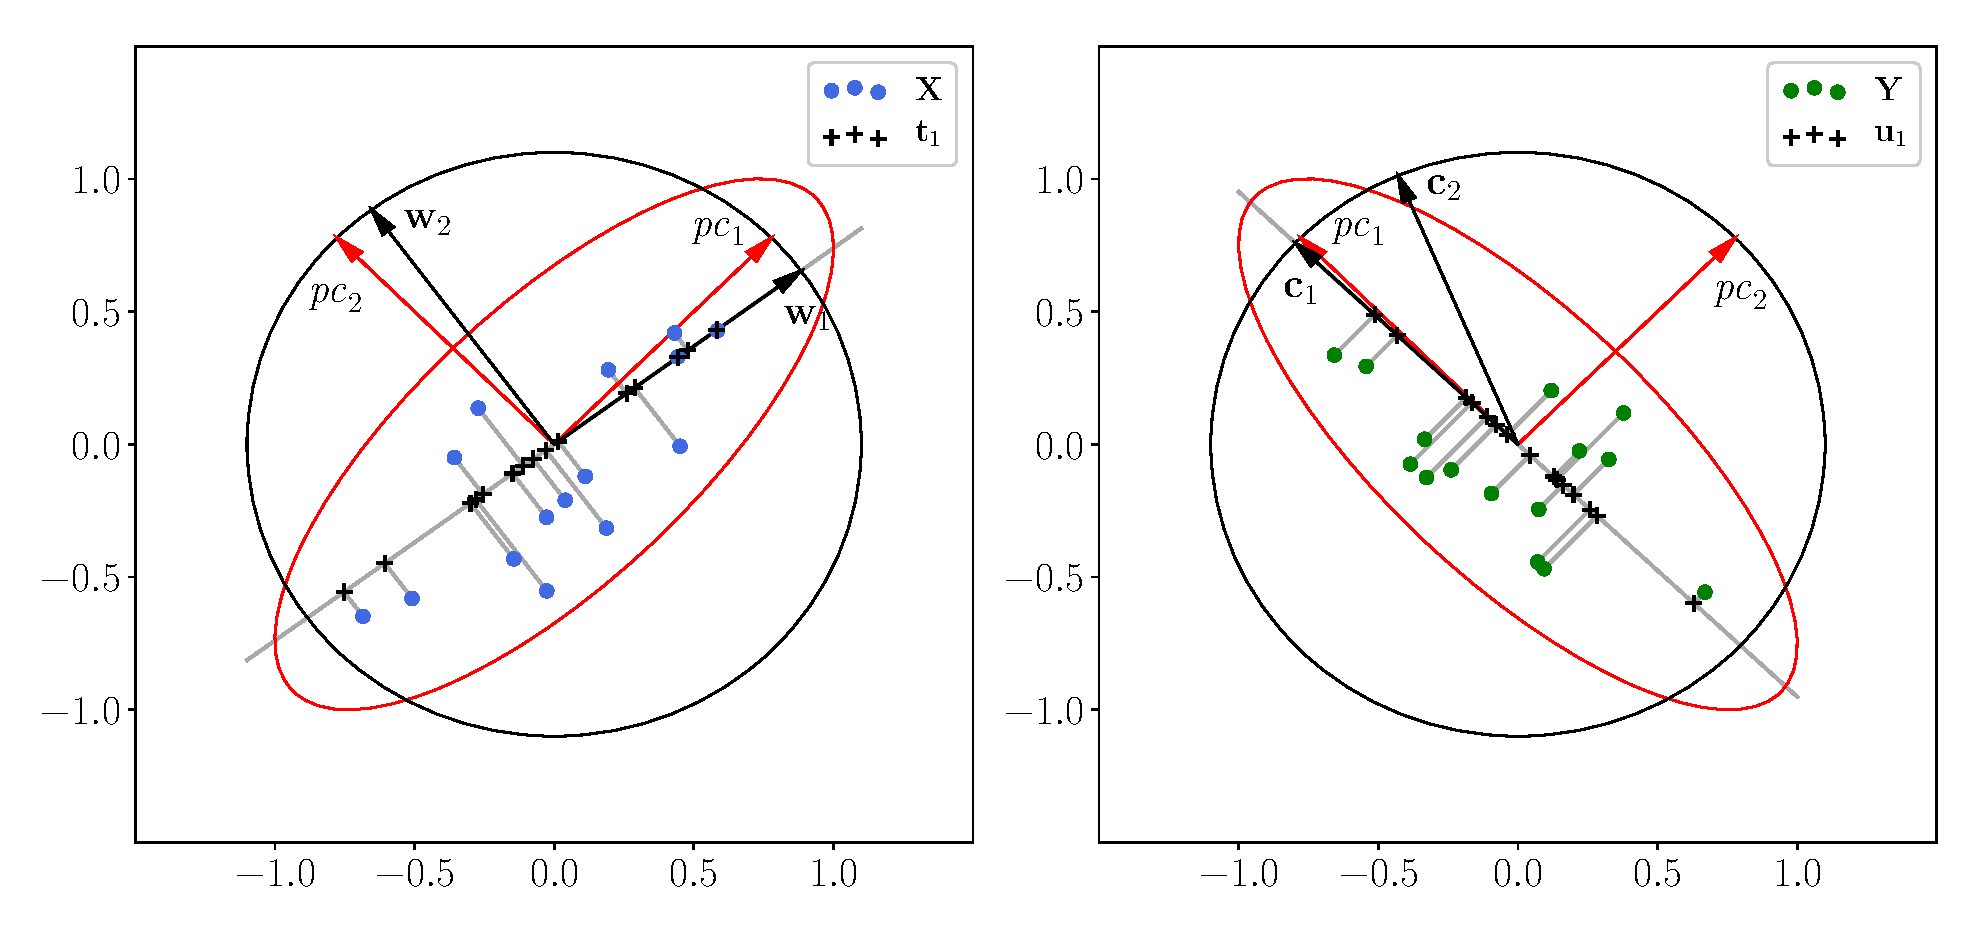
\includegraphics[width=\linewidth]{figs/PLSFigure.eps}
	\caption{Иллюстрация алгоритма PLS}
	\label{fig::PLSFigure}
\end{figure}

Для получения прогнозов модели и нахождения параметров модели 
домножим справа формулу~\eqref{eq::PLS_X} на матрицу $\bW$. Строки матрицы невязок $\bE$ ортогональны столбцам матрицы $\bW$, поэтому 
\[
	\bX \bW = \bT \bP^{\T} \bW.
\] 
Линейное преобразование между объектами в исходном и латентном пространстве имеет вид
\begin{equation}
	\bT = \bX \bW^*,
	\label{eq::W*}
\end{equation}
где $\bW^* = \bW (\bP^{\T} \bW)^{-1}$. 

Матрица параметров модели~\ref{eq::model} находится из уравнений~\eqref{eq::PLS_Y},~\eqref{eq::W*}
\begin{equation*}
    \bY = \bT \bQ^{\T} + \bE = \bX \bW^* \bQ^{\T} + \bE = \bX \bTheta + \bE.
\end{equation*}
Таким образом, параметры модели~\eqref{eq::model} равны
\begin{equation}
    \bTheta = \bW (\bP^{\T} \bW)^{-1} \bQ^{\T}.
    \label{eq::model_parameters}
\end{equation}
После нахождения параметров модели на этапе тестирования для нахождения предсказания модели необходимо
\begin{itemize}
	\item нормировать тестовые данные;	
	\item вычислить предсказание модели с помощью линейного преобразования с матрицей $\bTheta$ из~\eqref{eq::model_parameters};
	\item провести обратную нормировку.
\end{itemize}

%%%%%%%%%%%%%%%%%%%%%%%%%%%%%%%%%%%%%%%%%%%%%%%%%%%%%%%%%%%%%%%%%%%%%%%%%%%%%%
\section{Вычислительный эксперимент}
%%%%%%%%%%%%%%%%%%%%%%%%%%%%%%%%%%%%%%%%%%%%%%%%%%%%%%%%%%%%%%%%%%%%%%%%%%%%%%
Временные ряды энергии состоят из почасовых записей (всего 52512 наблюдений), а погодные измерения проводились раз в день и содержат 2188 наблюдений. 
Строка матрицы $\bX$~--– локальная история сигнала за одну неделю $n = 24 \times 7$. Строка матрицы $\bY$~--- локальный прогноз потребления электроэнергии в следующие 24 часа $r = 24$. В этом случае матрицы $\bX$ и $\bY$ являются авторегрессионными матрицами(можно ссылку).

В случае данных ECoG матрица $\bX$ состоит из пространственно-временного спектрального представления временных рядов напряжения, а матрица $\bY$ содержит информацию о положении руки. 
Процесс генерации матрицы $\bX$ из значений напряжения описан в~\cite{gasanov2017pls}. 
Признаковое описание в каждый момент времени имеет размерность $864$, положение руки описывается координатами по трём осям. 
Пример данных напряжения с разных каналов и соответствующих пространственных координат руки представлен на Рис.~\ref{fig::ecog_data}.
Для прогнозирования движения руки используется авторегрессионный подход.
Один объект состоит из признакового описания в несколько отсчётов времени. 
Ответом является положение руки в несколько следующих моментов времени.
Требуется предсказать положение руки в несколько следующих моментов времени.

\begin{figure}
	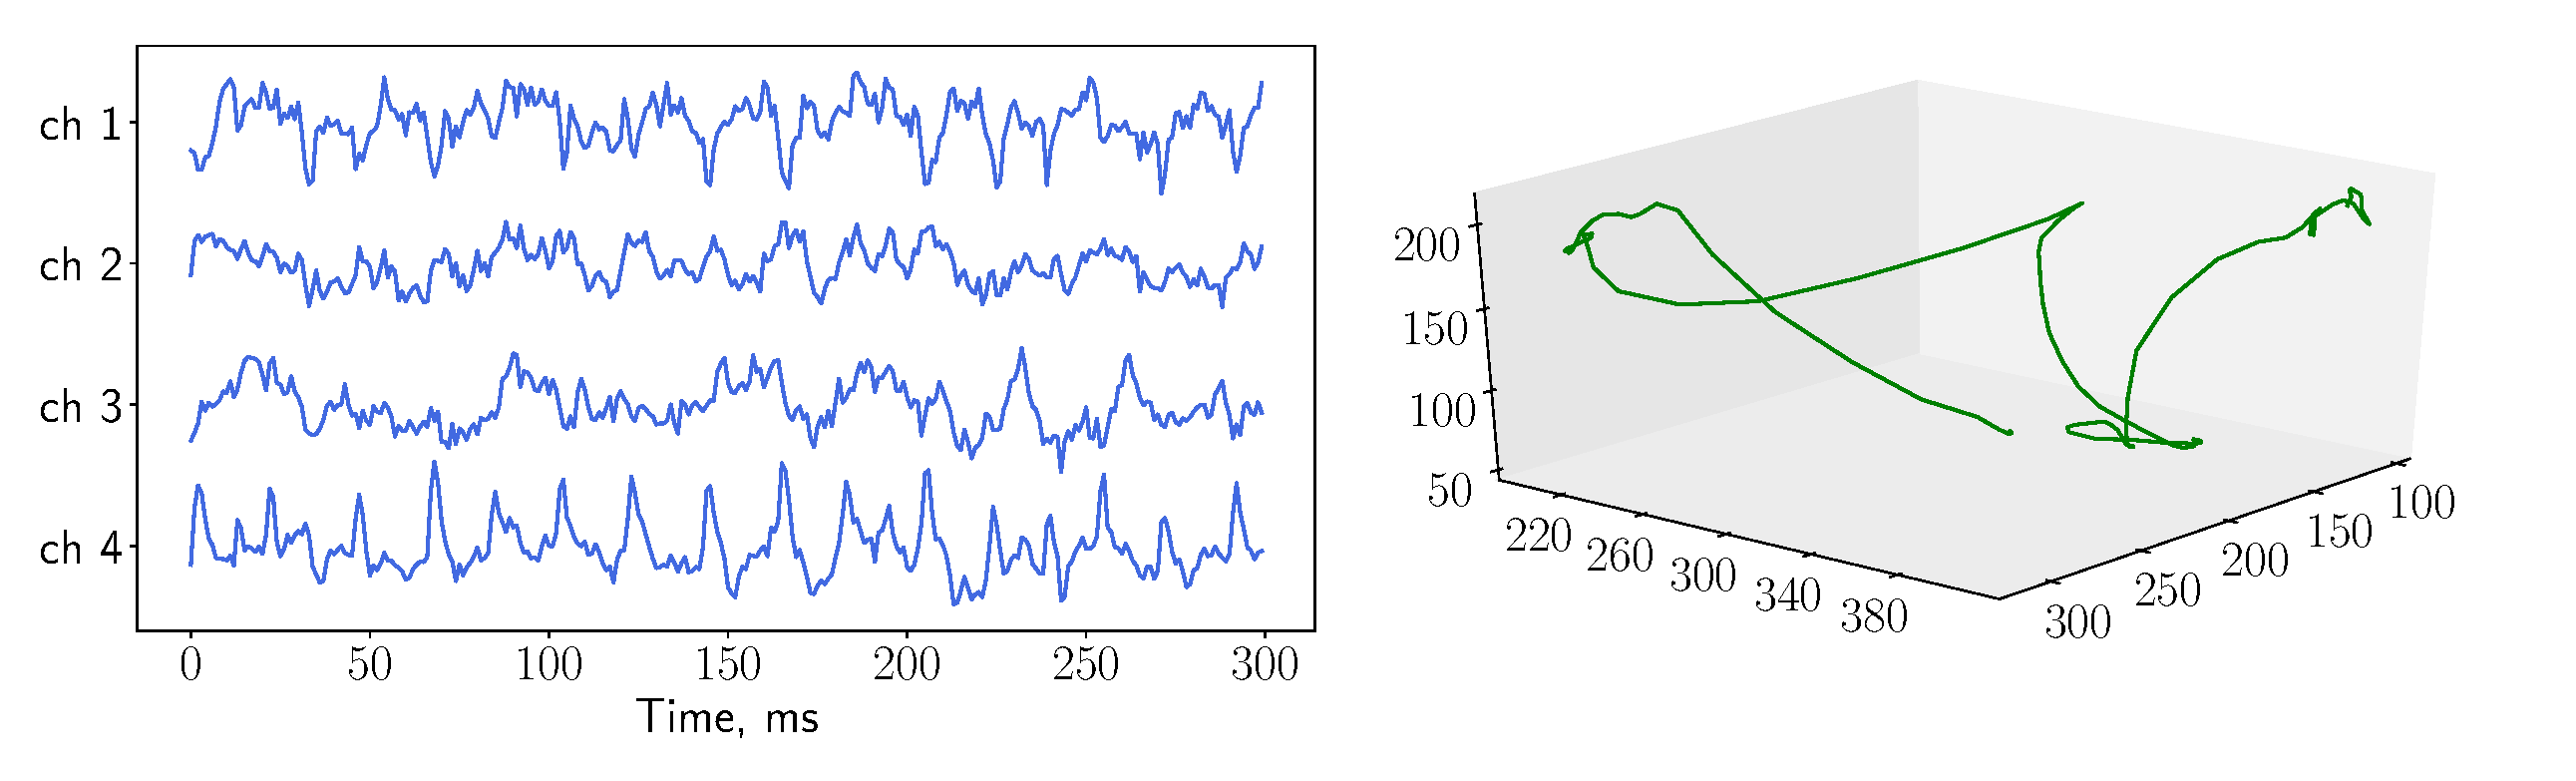
\includegraphics[width=\linewidth]{figs/ecog_data.eps}
	\caption{Пример данных ECoG. Слева изображены данные напряжения снятые с нескольких каналов, справа~--- координаты руки по трём осям.}
	\label{fig::ecog_data}
\end{figure}

Введём среднеквадратичную ошибку для некоторых матриц $\mathbf{A} = [a_{ij}]$ и $\mathbf{B} = [b_{ij}]$
\[
\text{MSE} (\mathbf{A}, \mathbf{B}) = \sum_{i,j} (a_{ij} - b_{ij})^2.
\]
Для оценивания качества аппроксимации вычисляется значение нормированной среднеквадратичной ошибки
\begin{equation}
\text{NMSE}(\bY,  \mathbf{\hat{Y}}) = \frac{\text{MSE} (\bY, \mathbf{\hat{Y}})}{\text{MSE} (\bY, \mathbf{\bar{Y}})},
\label{eq::nmse}
\end{equation}
где $\mathbf{\hat{Y}}$~--- прогноз модели, $\mathbf{\bar{Y}}$~--- константный прогноз средним значением по столбцам матрицы.

\subsection{Данные потребления электроэнергии}

Для нахождения оптимальной размерности $l$ латентного пространства все данные потребления электроэнергии были разбиты на обучающую и валидационную части. 
Обучающая выборка состоит из $700$ объектов, валидационная из $370$. Зависимость нормированной квадратичной ошибки~\eqref{eq::nmse} от размерности $l$ латентного пространства представлена на Рис.~\ref{fig::energy_n_comp}. 
Сначала ошибка резко падает при увеличении размерности скрытого пространства, а затем меняется незначительно.

\begin{figure}[!h]
	\centering
	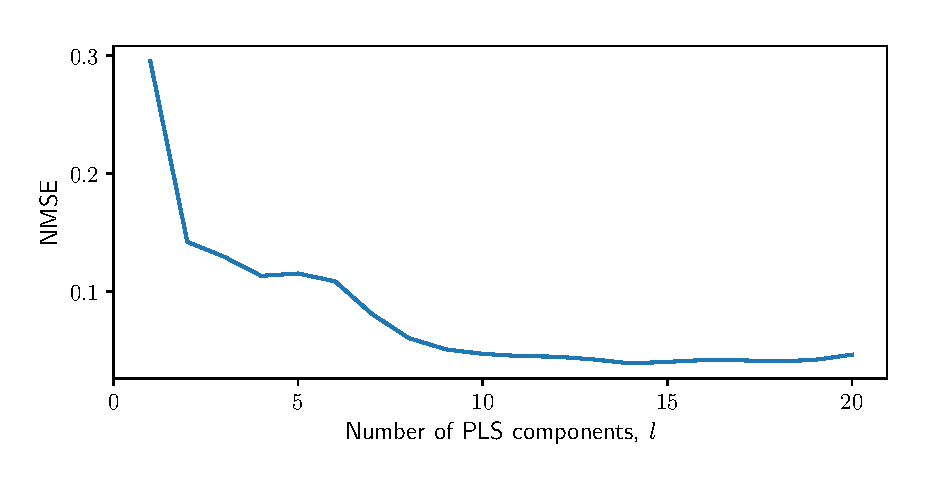
\includegraphics[width=0.75\linewidth]{figs/energy_n_comp}
	\caption{Прогноз потребления электроэнергии алгоритмом PLS при размерности латентного пространства $l$=14}
	\label{fig::energy_n_comp}
\end{figure}

Минимальная ошибка наблюдается при $l=14$. 
Построим прогноз потребления электроэнергии при данном $l$. 
Результат аппроксимации изображен на Рис.~\ref{fig::energy_prediction}. Алгоритм PLS восстановил авторегрессионную зависимость и обнаружил дневную сезонность.

\begin{figure}[!h]
	\centering
	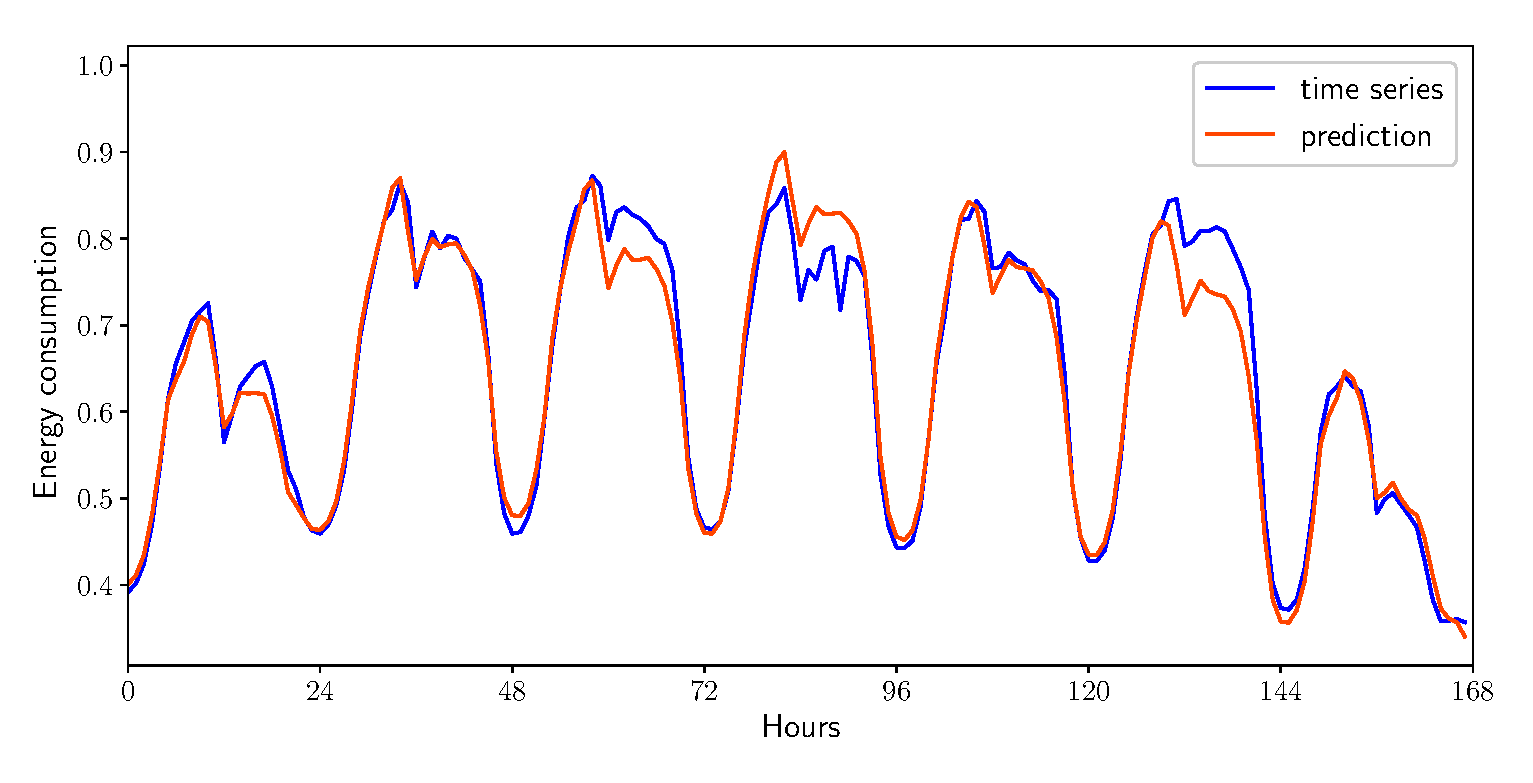
\includegraphics[width=0.95\textwidth]{figs/energy_prediction}
	\caption{Зависимость ошибки от размерности латентного пространства для данных потребления электроэнергии}
	\label{fig::energy_prediction}
\end{figure}

\subsection{Данные электрокортикограммы}

На Рис.~\ref{fig::ecog_n_comp} представлена зависимость нормированной квадратичной ошибки~\eqref{eq::nmse} от размерности латентного пространства. Ошибка аппроксимации меняется незначительно при $l > 5$.
Таким образом совместное описание пространственно-временного спектрального представления объектов и пространственного положения руки может быть представлено вектором размерности $l \ll n$.
Зафиксируем $l = 5$. 
Пример аппроксимации положения руки изображен на Рис.~\ref{fig::ecog_prediction}. 
Сплошными линиями изображены истинные координаты руки по всем осям, пунктирными линиями показана аппроксимация методом PLS.
 
\begin{figure}[!h]
	\centering
	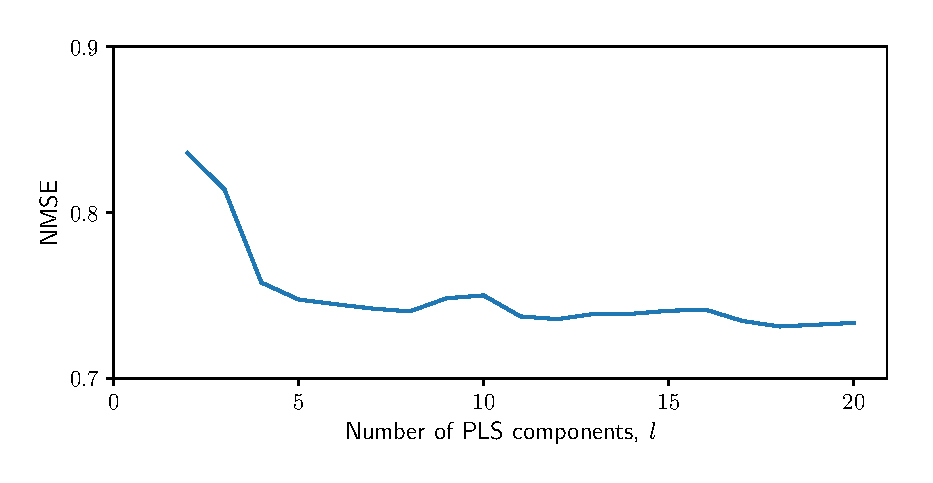
\includegraphics[width=0.75\linewidth]{figs/ecog_n_comp}	
	\caption{Зависимость ошибки от размерности латентного пространства для данных ECoG}
	\label{fig::ecog_n_comp}
\end{figure}

\begin{figure}[!h]
	\centering
	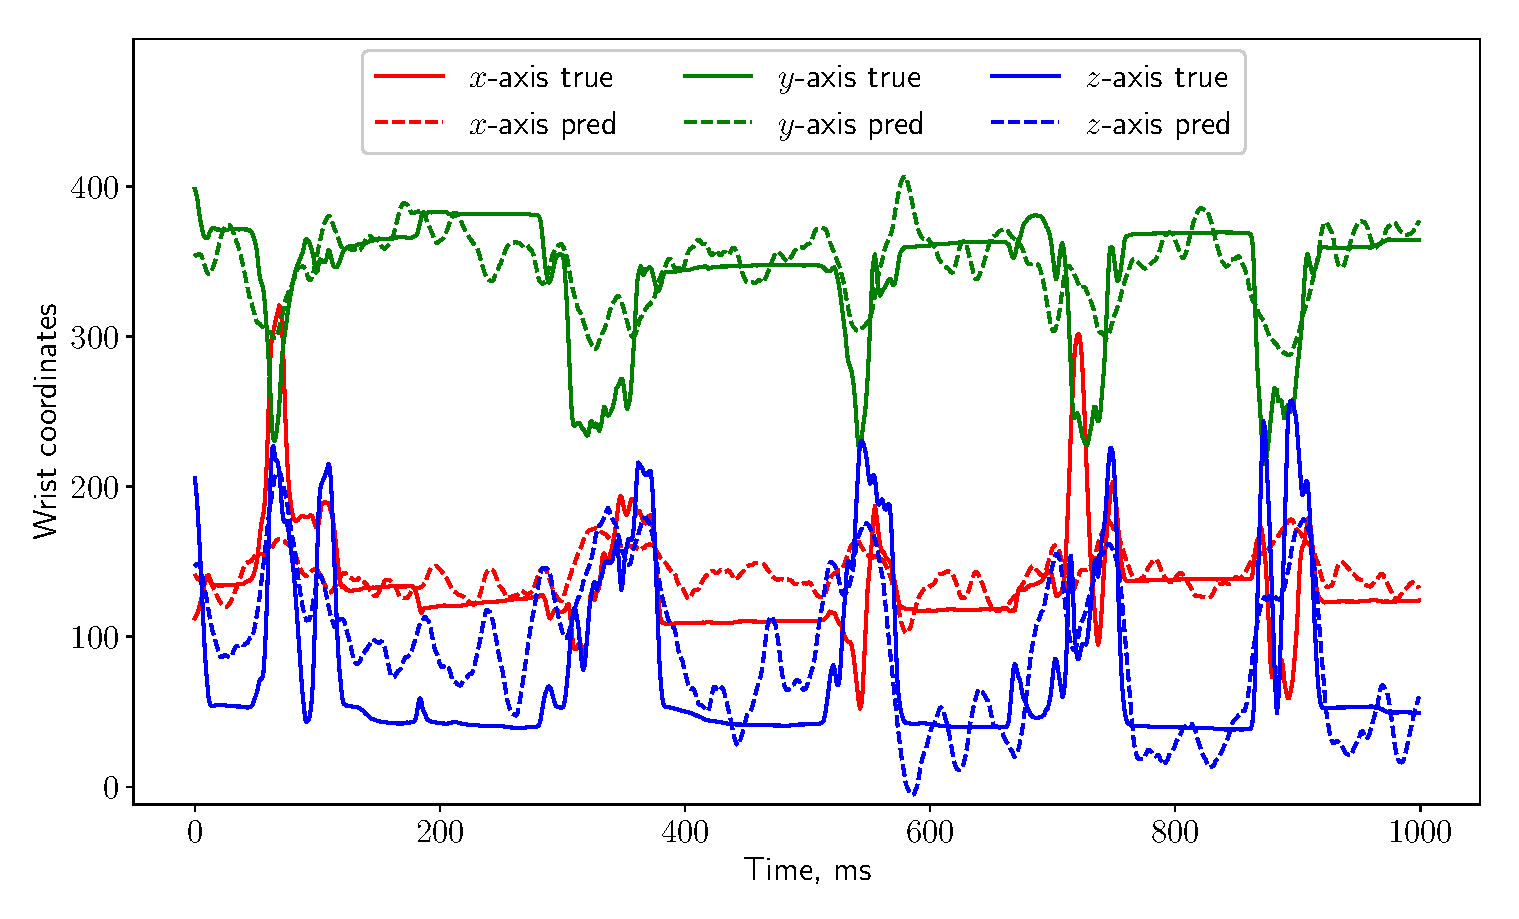
\includegraphics[width=\textwidth]{figs/ecog_prediction}
	\caption{Прогноз движения руки данных ECoG алгоритмом PLS при размерности латентного пространства $l=5$}
	\label{fig::ecog_prediction}
\end{figure}

%%%%%%%%%%%%%%%%%%%%%%%%%%%%%%%%%%%%%%%%%%%%%%%%%%%%%%%%%%%%%%%%%%%%%%%%%%%%%%
\section{Заключение}
В данной работе предложен новый подход к обнаружению зависимостей в пространстве зависимой переменной задачи прогнозирования временных рядов. Сравнивались результаты прогнозирования временных рядов, полученных с помощью метода частных наименьших квадратов и предложенной модификации. Проведен вычислительный эксперимент на реальных данных потребления электроэнергии в Варшаве. Построенная прогностическая модель показала высокое качество предсказания электрической нагрузки. 
%%%%%%%%%%%%%%%%%%%%%%%%%%%%%%%%%%%%%%%%%%%%%%%%%%%%%%%%%%%%%%%%%%%%%%%%%%%%%%
%\section*{СПИСОК ЛИТЕРАТУРЫ}

%\nocite{*}

\bibliographystyle{unsrt}
\bibliography{papers_pls}


\end{document}